\documentclass[10pt,twocolumn]{article}

\usepackage[margin=0.75in]{geometry}
\usepackage{graphicx}
\usepackage{booktabs}
\usepackage{array}
\usepackage{url}
\usepackage[hidelinks]{hyperref}

\graphicspath{{figures/}}
\setlength{\parskip}{0.25em}
\setlength{\parindent}{1em}

\title{\textbf{MARBTS: A Negotiating Multi-Agent Red/Blue Team Simulator for Safe Autonomous Cyber-Defense Experiments}}

\author{
\begin{tabular}{c}
Sargam Nema (1MS22CI057), Shobhit Srivastava (1MS22CI063),\\
Aryaman Prakash (1MS22CY010), Suryansh Prajapati (1MS22CY069)\\
\small Department of Computer Science and Engineering, Ramaiah Institute of Technology, Bengaluru, India
\end{tabular}
}

\date{Project paper prepared from the CIP81 report and implementation artifacts, 2025--2026}

\begin{document}
\maketitle

\begin{abstract}
Autonomous cyber-defense research needs environments where attacker and defender behavior can be studied without touching real infrastructure. MARBTS addresses this need through a sandboxed Red/Blue simulator that models a network as a graph, constrains both agents to abstract legal actions, and records every timestep with reproducible provenance. The system combines scenario validation, a turn-based simulation kernel, rule-based and adaptive policies, structured observability, metrics, comparative reports, stress testing, and ablation workflows. This paper rewrites and consolidates the CIP81 project report into a compact research-paper form while cross-checking implementation details against the repository. The verified results show that the rule baseline remains stable at zero final compromises, while adaptive Red behavior creates one compromised node in the baseline scenario and triggers two Blue containment actions under the same two-step horizon. Across the primary policy matrix, deterministic consistency remains 1.0, supporting repeatable experimentation under fixed seeds.
\end{abstract}

\textbf{Keywords---} cyber-defense simulation, red team, blue team, multi-agent systems, reproducibility, cyber range, adaptive planning.

\section{Introduction}
Red-team and blue-team exercises are useful for reasoning about attacker pressure and defensive response, but live exercises are difficult to repeat and risky to automate. A realistic experiment should let researchers vary network topology, policies, seeds, and observability while still preserving a complete explanation of what each actor did and why. MARBTS, the Negotiating Multi-Agent Red/Blue Team Simulator, was built for that controlled middle ground: it is not an exploitation framework, but a safe experimental system for studying interactions between abstract offensive and defensive agents.

The central idea is to represent a cyber environment as a validated graph. Nodes represent assets such as servers, databases, IoT devices, or endpoints. Edges represent connectivity. Red agents can scan, exploit, escalate, and move laterally when those actions are legal. Blue agents can monitor, patch, block, and isolate. The simulation kernel alternates Red and Blue turns, applies state transitions, and writes structured artifacts that can be replayed, compared, and summarized.

This paper treats the submitted CIP81 report as the source of truth for project intent, requirements, and reported findings \cite{cip81}. The repository is used only as a consistency check for implementation names, package paths, command-line entry points, dependency versions, and metric artifacts. That check corrected one report-level naming drift: the CLI package is implemented as \path{src/marbts_cli/}, not \path{src/marbtscli/}.

\section{Problem and Objectives}
The project targets a gap between high-fidelity cyber ranges and small hand-written examples. Existing platforms can emulate adversaries or train defenders, but a course-scale research prototype also needs to be lightweight, inspectable, deterministic under seeds, and explicit about causal state changes. The problem is therefore to build a controlled simulator where every action is legal by construction, every decision has a rationale, and every run can be compared against another run without hidden side effects.

The main objectives are:
\begin{itemize}
\item Model synthetic enterprise networks as schema-validated graphs with explicit node attributes and connectivity.
\item Provide safe abstract actions for Red and Blue agents without live exploit tooling, network interaction, or real target systems.
\item Implement deterministic rule-based baselines and adaptive planning policies behind a common policy interface.
\item Record rationales, expected effects, state differences, hashes, seeds, and provenance for reproducible analysis.
\item Generate multi-seed, policy-matrix, stress-test, ablation, replay, visualization, and comparative-report artifacts.
\item Package the project through scripts, CLI commands, container support, notebooks, tests, and release-readiness checks.
\end{itemize}

\section{Related Work}
MARBTS is closest to cyber-range and adversary-emulation work, but it deliberately chooses a safer abstraction level. MITRE CALDERA and automated adversary-emulation research demonstrate how repeatable adversary behavior can support security evaluation \cite{miller,caldera}. Cyber ranges and simulation surveys motivate the need for training and experimentation environments that can be reset, instrumented, and scaled \cite{priya,javadpour}. Reinforcement-learning and adaptive-defense studies show how autonomous policies can be evaluated under controlled assumptions \cite{wang,morozov}. Recent work on deception, LLM-assisted cyber agents, and autonomous cyber operations provides useful context, but MARBTS keeps model routing optional and falls back to heuristic planning in the checked-in baseline \cite{landolt,xie,soule}.

\section{Scope and Requirements}
The system scope is intentionally bounded. MARBTS simulates decisions and state transitions; it does not execute malware, run exploit frameworks, attack real hosts, or require external network access during simulation. This boundary is important because it allows experimentation with attacker-defender dynamics while keeping the environment safe for coursework and reproducible research.

The implementation targets Python 3.11 or later. The checked project metadata lists \texttt{networkx} for graph handling, \texttt{matplotlib} for visualization, and \texttt{packaging} for release/runtime checks; development tests use \texttt{pytest}. The report recommends a modern laptop-class CPU, at least 8 GB RAM, and Linux, Windows, or macOS. Docker, shell tooling, and notebooks are supported for packaging and analysis, but the core simulator is command-line and artifact driven rather than a web application.

Functionally, the project must load scenarios, validate schemas, build runtime graphs, enumerate legal actions, run turn-based Red/Blue simulations, select actions through rule or adaptive policies, serialize logs, compute metrics, and generate reports. Non-functional requirements emphasize safety, reproducibility, explainability, modularity, maintainability, scalability, testability, portability, and research utility.

\section{System Design}
Figure~\ref{fig:architecture} summarizes the report-level architecture. Inputs enter through scenario files, experiment configurations, and runtime presets. Scenario validation creates typed objects, the environment layer builds the graph and legal action space, the simulation kernel executes Red/Blue turns, and the observability layer writes replayable artifacts. Metrics, visualization, and experiment runners then turn those artifacts into reports.

\begin{figure*}[t]
\centering
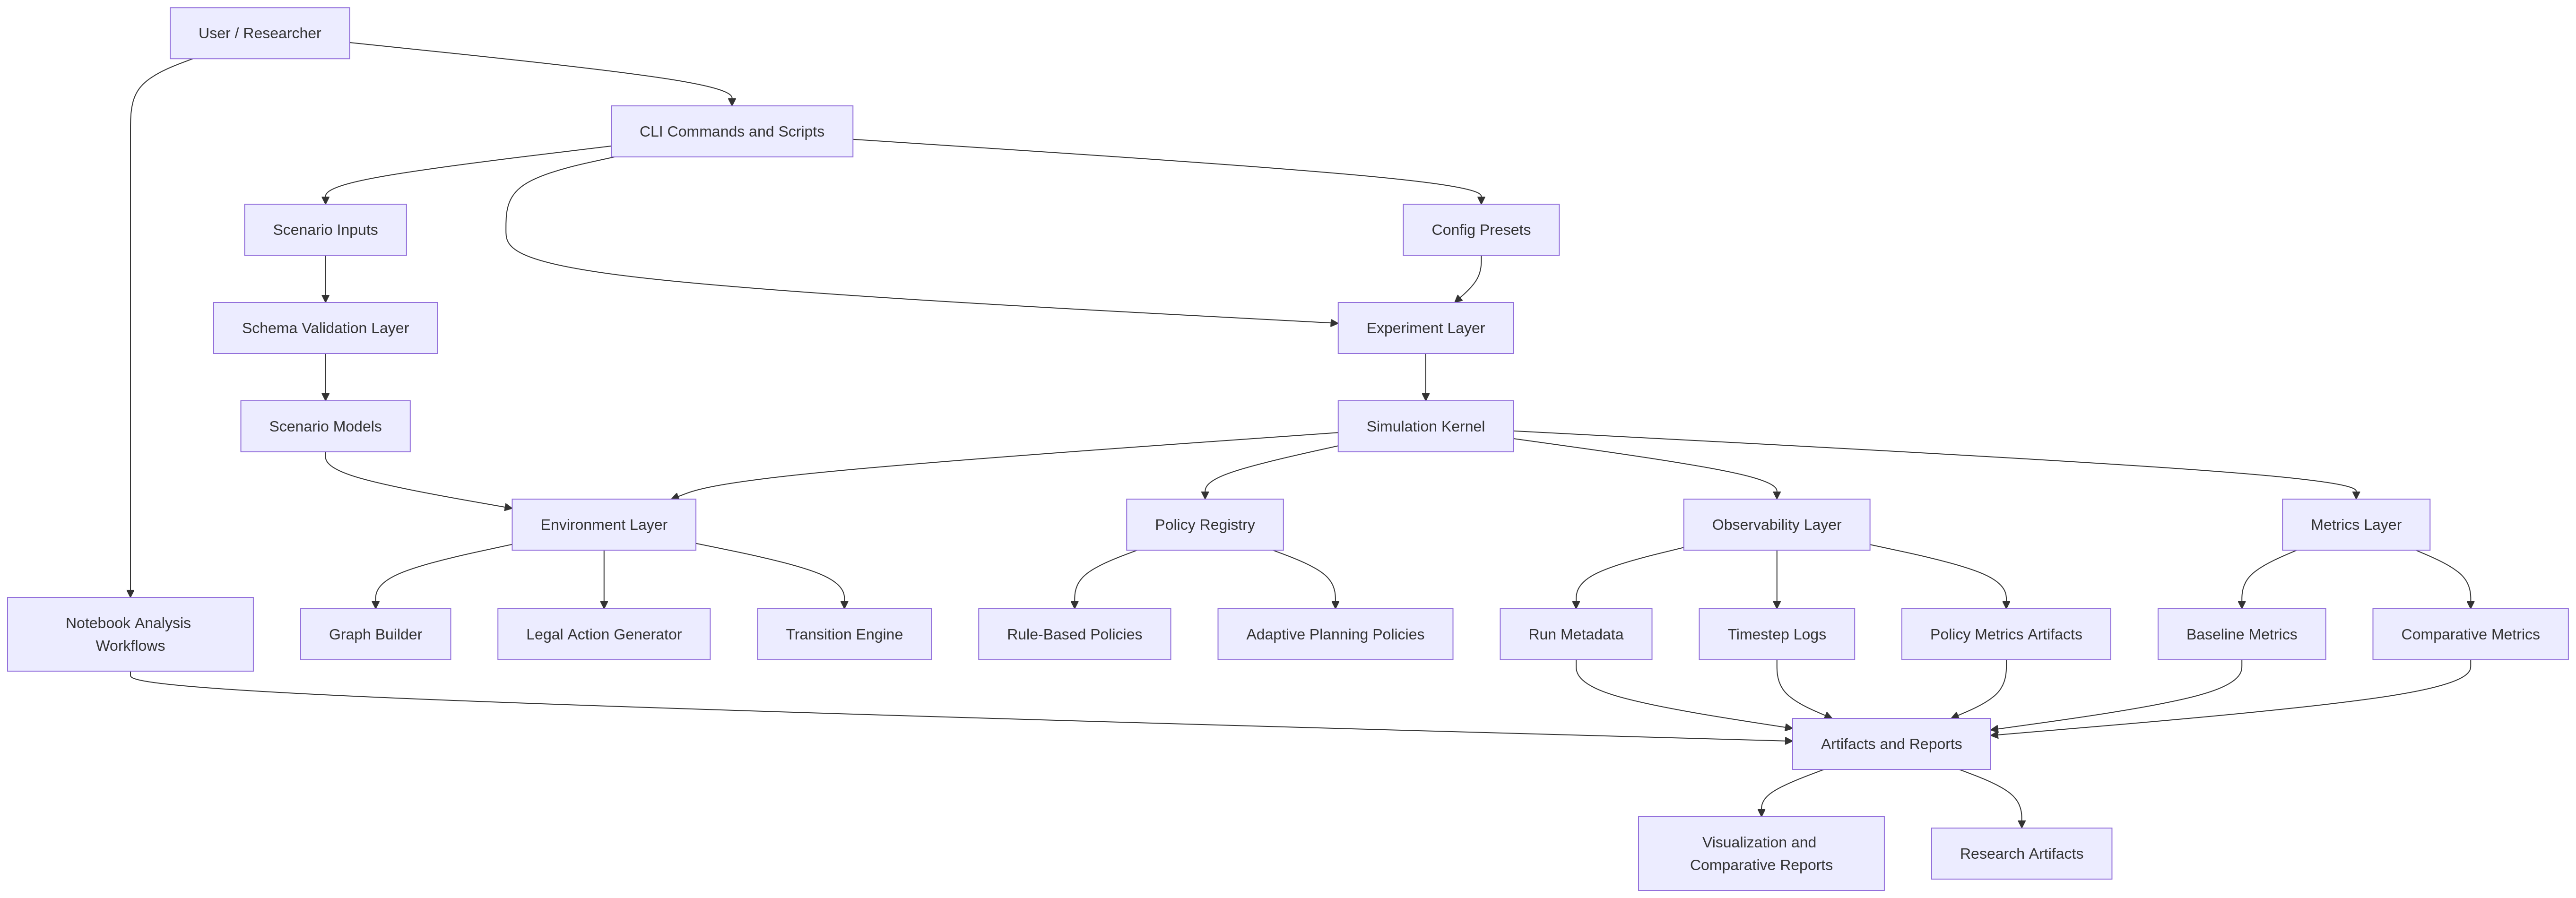
\includegraphics[width=\textwidth]{report_architecture.png}
\caption{Report-derived architecture view of MARBTS. The implementation check confirms the same layered structure, with the CLI package located at \path{src/marbts_cli/}.}
\label{fig:architecture}
\end{figure*}

The implementation is organized around clear module boundaries. Shared enums and models live under \path{src/hart/}. Scenario validation and catalog support are implemented under \path{src/schemas/}. The environment layer contains graph construction, state storage, legal-action enumeration, and transitions. Agent packages contain rule-based Red and Blue policies plus adaptive planning, deception hooks, and optional model routing. The simulation layer owns seeded execution, policy context construction, state diffs, and timestep logs. Observability, metrics, experiments, visualization, and CLI packages handle downstream analysis and delivery.

The low-level runtime state includes node type, services, vulnerabilities, security level, compromised state, detection state, and isolation state. The verified enum values include \texttt{server}, \texttt{database}, \texttt{iot}, and \texttt{endpoint} node types; compromised states \texttt{none}, \texttt{user}, and \texttt{privileged}; and detection states \texttt{undetected}, \texttt{suspected}, and \texttt{confirmed}. Current baseline transitions mutate compromise, security, isolation, and connectivity; scan and monitor are informational actions in the kernel and do not directly mutate the graph.

\begin{figure}[t]
\centering
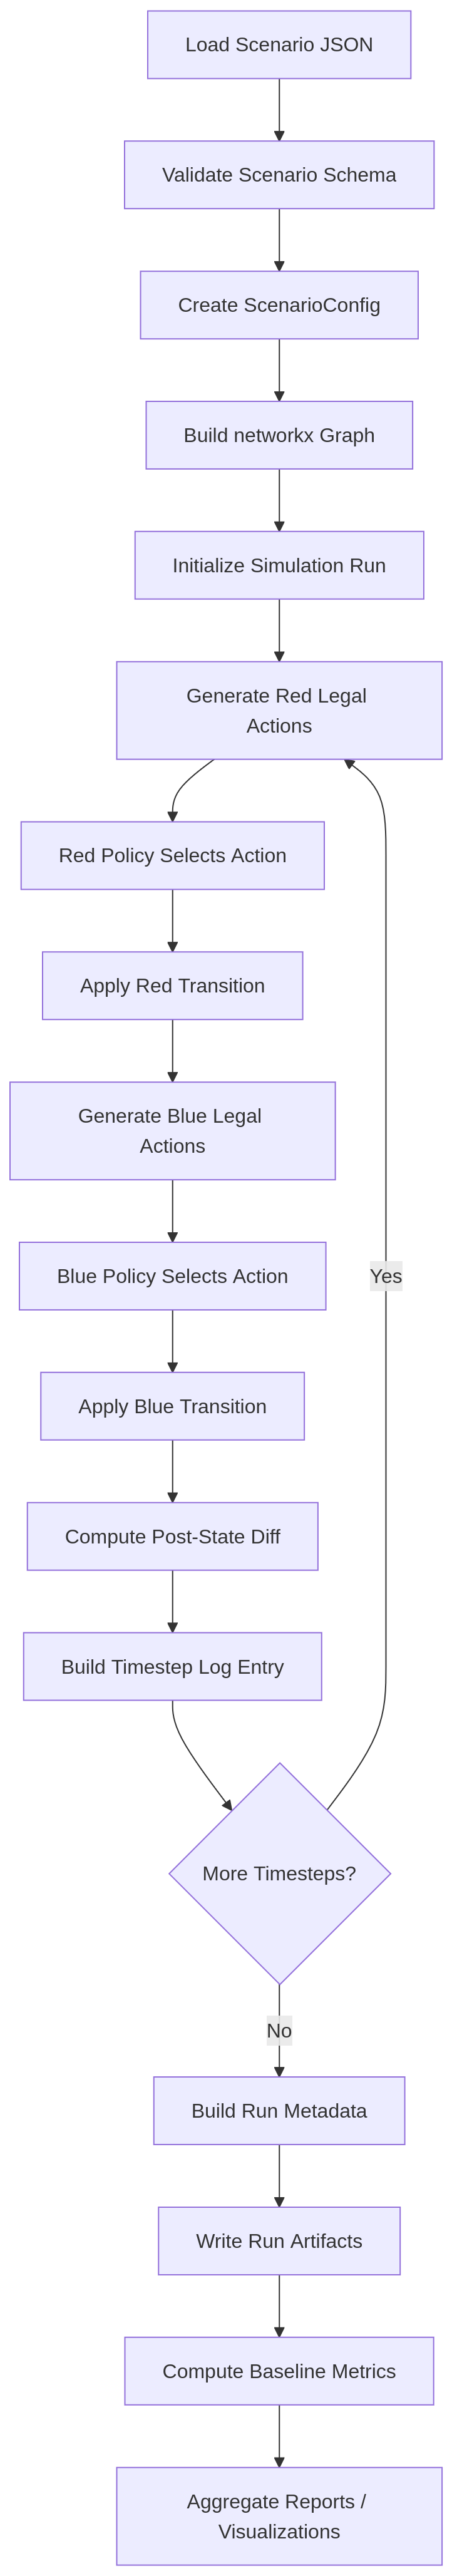
\includegraphics[width=\linewidth]{report_runtime_flow.png}
\caption{Runtime execution flow from scenario loading through per-timestep simulation and artifact generation.}
\label{fig:runtime}
\end{figure}

\section{Implementation}
The simulator starts by parsing a scenario dictionary or JSON file into validated nodes and edges. The graph builder copies validated attributes into a NetworkX graph. Legal-action generation then filters actions by actor and state: Red receives scan actions for non-isolated nodes, exploit actions for vulnerable targets that are not already privileged, escalation actions for user-level footholds, and lateral-movement actions from compromised nodes to reachable neighbors. Blue receives monitor, patch, isolate, and edge-block actions where legal.

The transition functions are intentionally simple and inspectable. \texttt{apply\_exploit} advances a target one compromise level unless it is isolated or already maximally compromised. If the kernel enables exploit resistance, the same function uses a seeded random number generator and security-level-dependent success probability; otherwise the checked baseline exploit succeeds deterministically. \texttt{apply\_patch} increases security level, reduces compromise level by one, and removes one vulnerability when available. \texttt{apply\_isolate} marks a node isolated and removes its incident edges. \texttt{apply\_block} removes a selected edge.

Policy decisions are represented through a common interface containing a selected action, a rationale, expected effect metadata, and policy metrics. Rule policies provide deterministic baselines. Adaptive policies use heuristic planning by default and expose configuration for planning horizon, observability reduction, deception bias, decoys, bluffing, and model routing. In the verified baseline configuration, remote model routing is disabled and heuristic fallback is enabled.

The CLI exposes \texttt{marbts} plus specialized entry points for multi-seed reports, policy experiment matrices, stress tests, ablation reports, container profiles, and release validation. The report describes a CLI and notebook interface rather than a graphical desktop or web UI, and the repository matches that scope.

\begin{figure}[t]
\centering
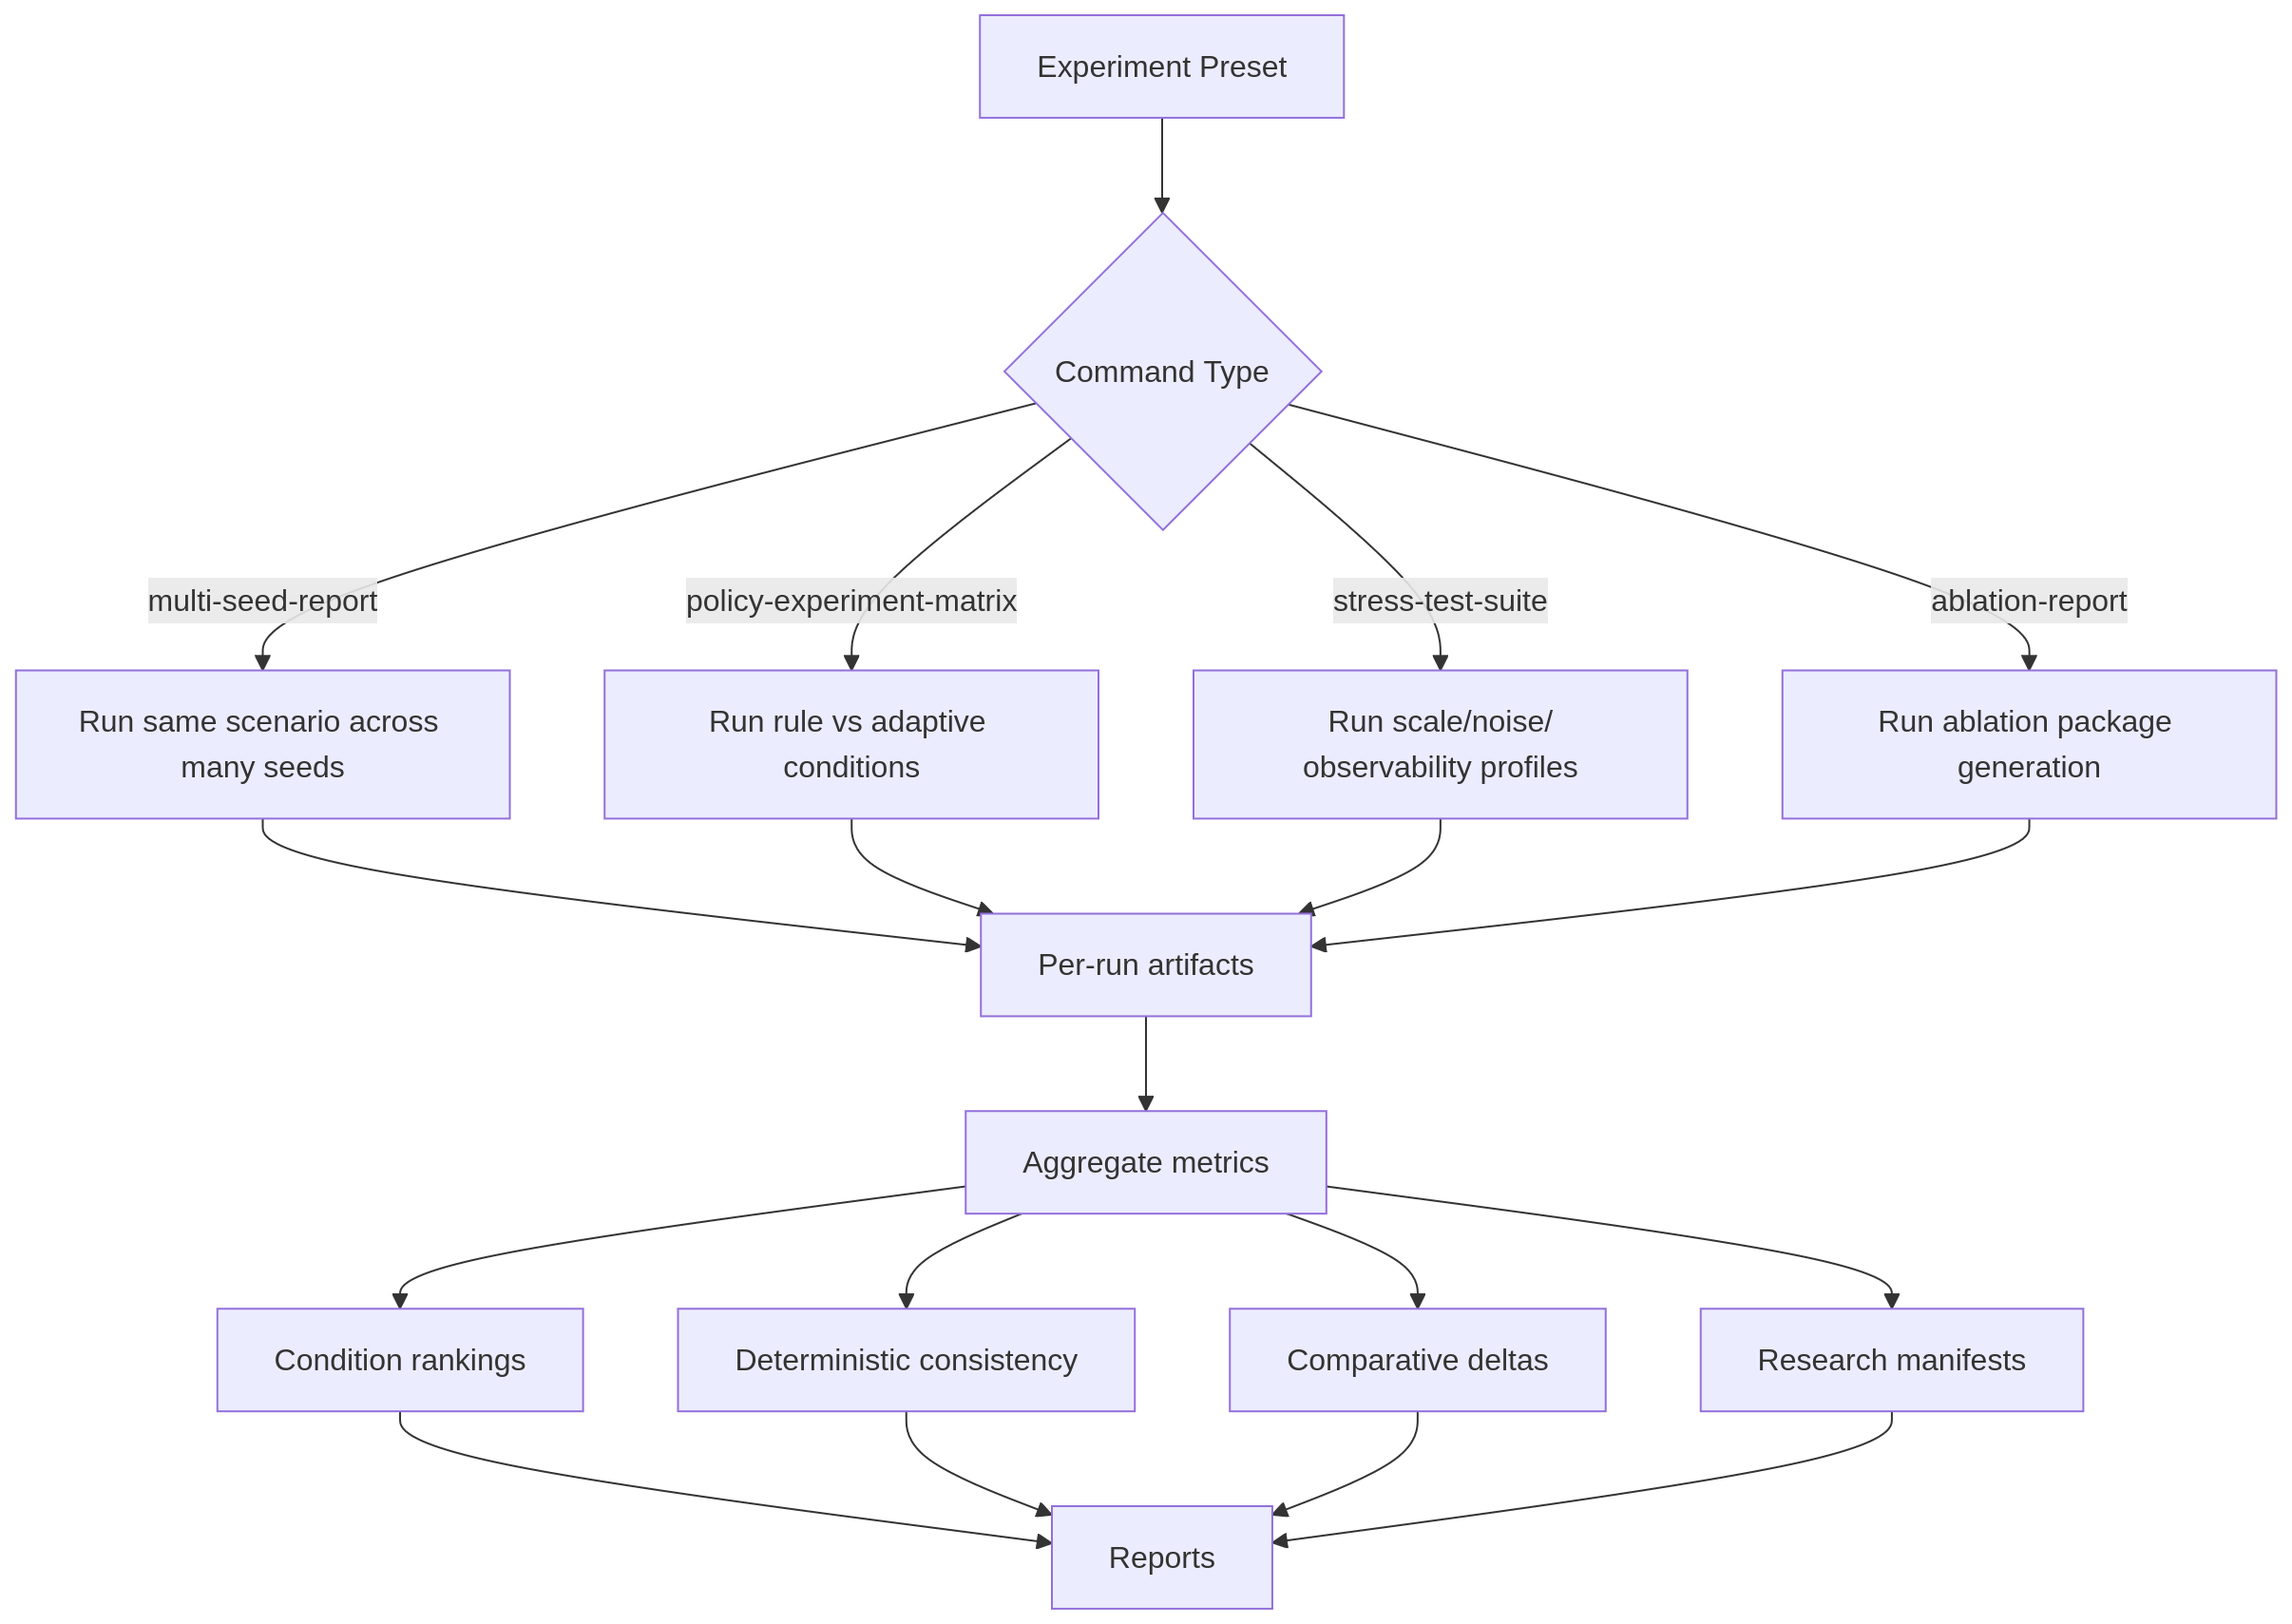
\includegraphics[width=\linewidth]{report_experiment_workflow.png}
\caption{Experiment and reporting workflow used to produce multi-seed, policy-matrix, stress-test, ablation, and comparative artifacts.}
\label{fig:workflow}
\end{figure}

\section{Experimental Results}
The primary report evaluates the \texttt{rule-baseline} scenario with fixed seeds and short horizons so that action traces can be inspected manually. Table~\ref{tab:single} shows the two-run comparison highlighted in the report and confirmed in the checked artifacts. With seed 20260423 and horizon 2, the rule baseline scans and monitors without changing graph state. Adaptive Red versus rule Blue exploits the IoT node twice, reaching one compromised node while Blue blocks two edges.

\begin{table}[t]
\centering
\caption{Two-run baseline comparison under seed 20260423 and horizon 2.}
\label{tab:single}
\begin{tabular}{@{}p{0.35\linewidth}ccc@{}}
\toprule
Condition & Final compromised & Blue containment & First containment \\
\midrule
Rule Red vs Rule Blue & 0 & 0 & N/A \\
Adaptive Red vs Rule Blue & 1 & 2 & 0 \\
\bottomrule
\end{tabular}
\end{table}

\begin{figure}[t]
\centering
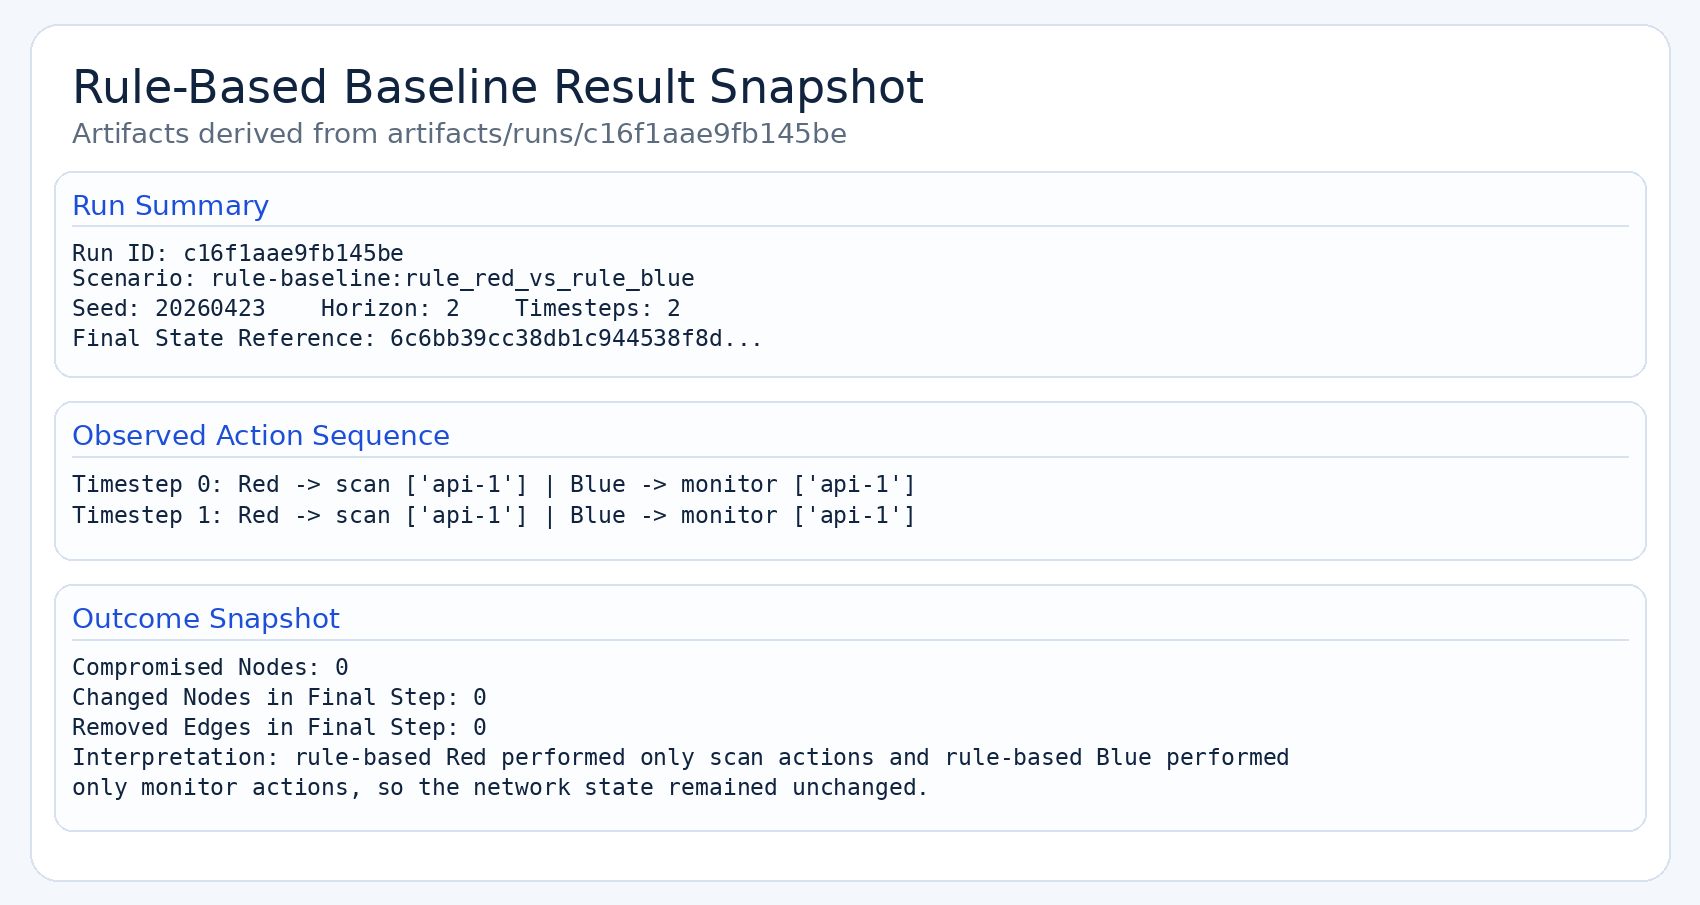
\includegraphics[width=\linewidth]{baseline_snapshot.png}
\caption{Baseline rule-policy snapshot from the report artifacts.}
\label{fig:baseline}
\end{figure}

\begin{figure}[t]
\centering
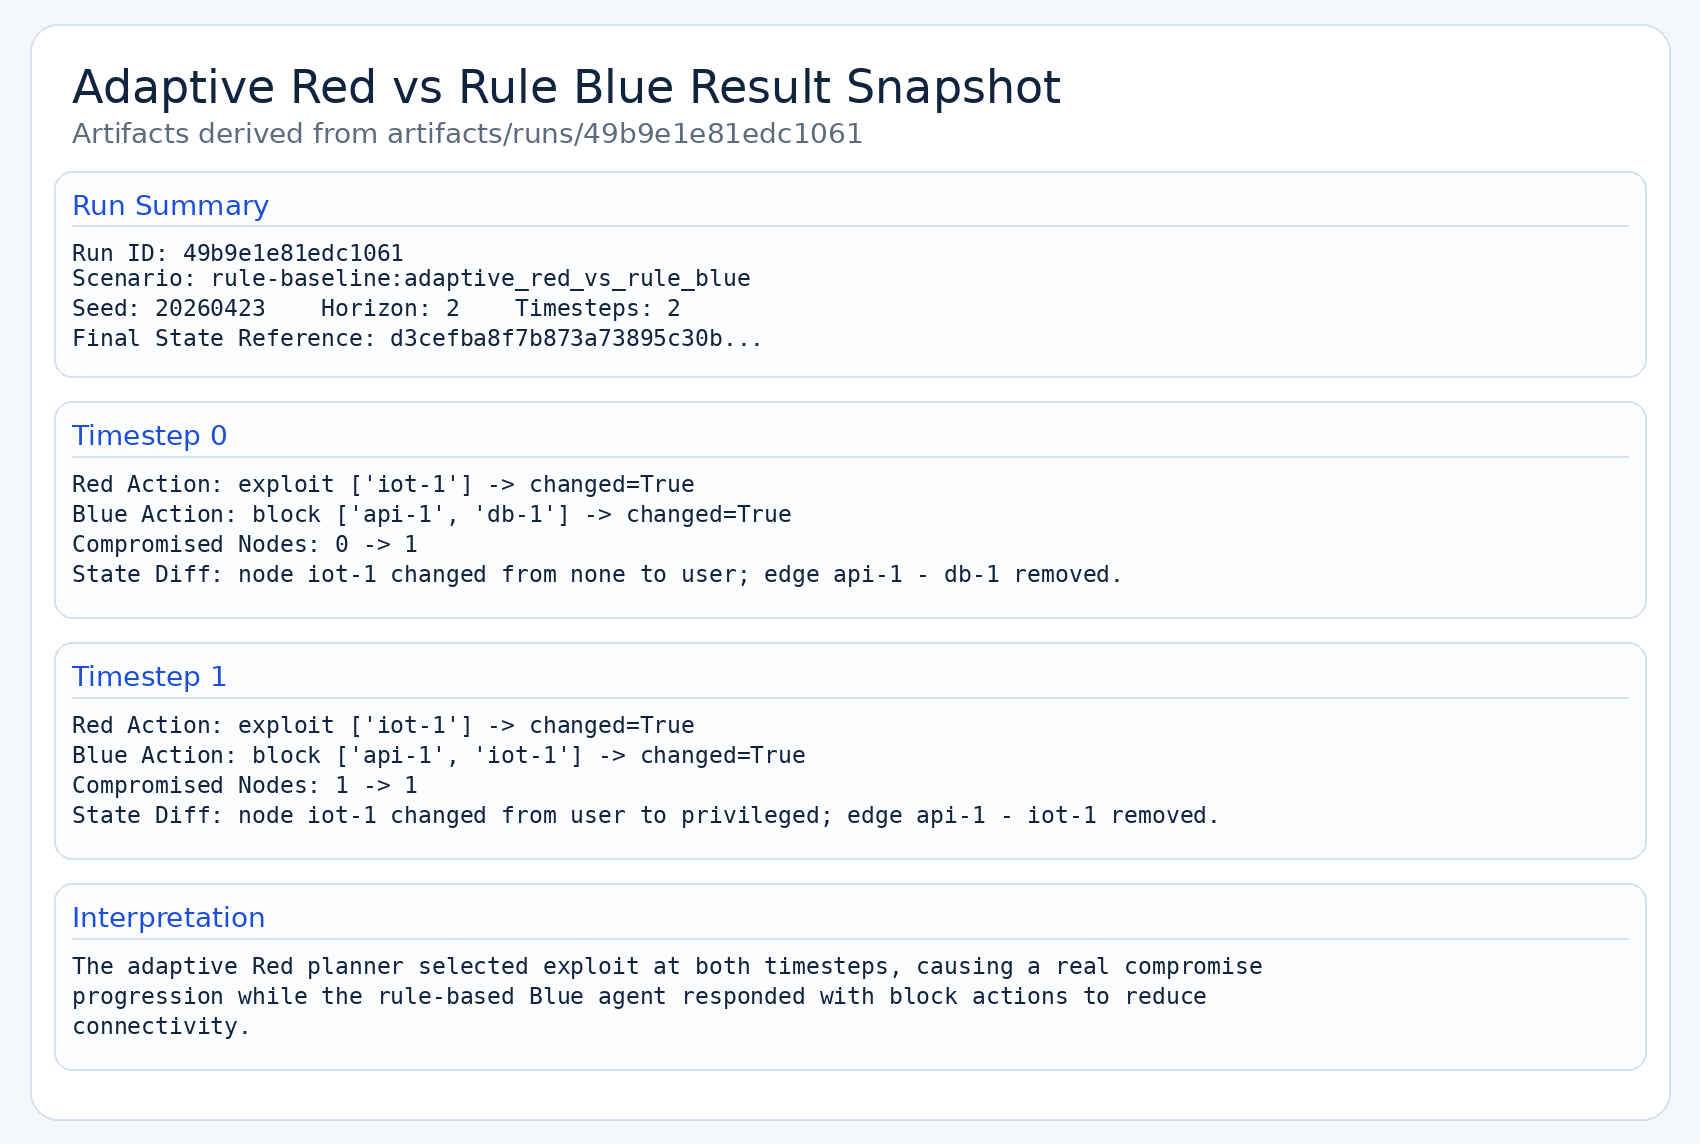
\includegraphics[width=\linewidth]{adaptive_red_snapshot.png}
\caption{Adaptive Red versus rule Blue snapshot, showing exploitation activity and Blue containment actions.}
\label{fig:adaptive}
\end{figure}

The multi-seed baseline report uses three seeds, horizon 8, and scenario version 1.0.0. It reports final compromised mean 0.0, final compromised standard deviation 0.0, Blue containment mean 0.0, and deterministic consistency ratio 1.0. This supports the intended role of the rule baseline as a stable reference condition.

Table~\ref{tab:matrix} gives the primary policy matrix. Adaptive Red increases final compromise under the tested baseline horizon. Adaptive Blue alone does not change the zero-compromise result when Red remains rule based. All four primary conditions remain deterministic across the two reported seeds.

\begin{table*}[t]
\centering
\caption{Primary policy matrix for \texttt{rule-baseline}, seed count 2, horizon 2.}
\label{tab:matrix}
\begin{tabular}{@{}lccc@{}}
\toprule
Condition & Final compromised mean & Blue containment mean & Deterministic consistency \\
\midrule
Rule Red vs Rule Blue & 0.0 & 0.0 & 1.0 \\
Adaptive Red vs Rule Blue & 1.0 & 2.0 & 1.0 \\
Rule Red vs Adaptive Blue & 0.0 & 0.0 & 1.0 \\
Adaptive Red vs Adaptive Blue & 1.0 & 0.0 & 1.0 \\
\bottomrule
\end{tabular}
\end{table*}

\begin{figure}[t]
\centering
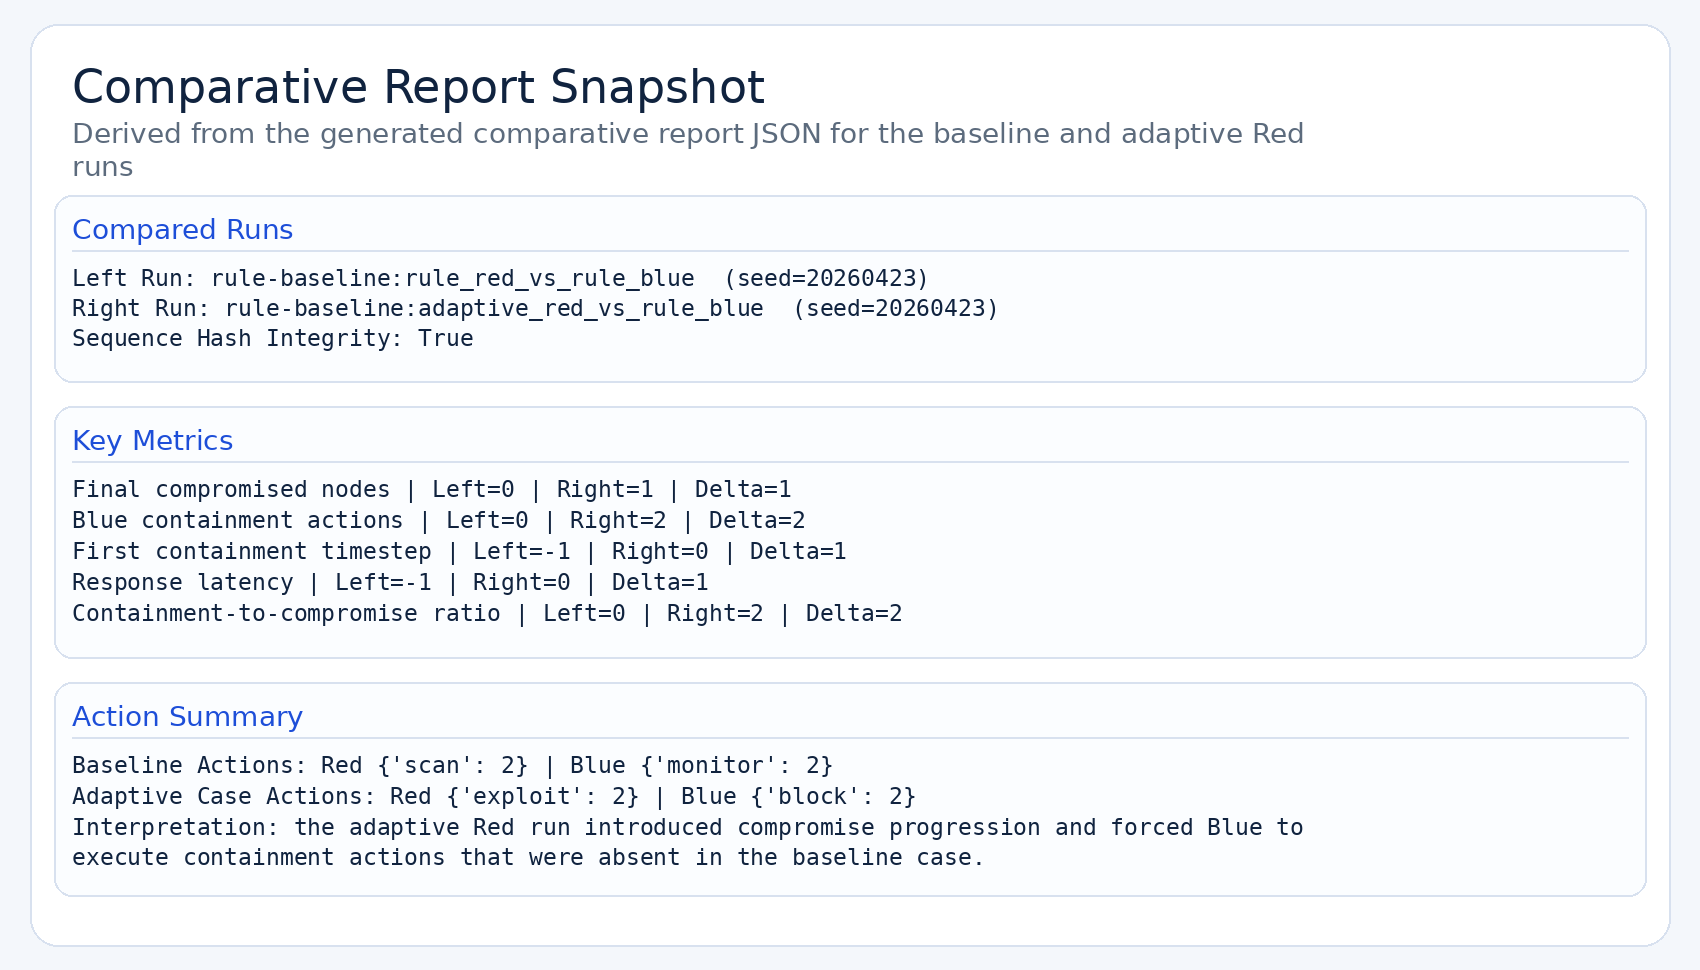
\includegraphics[width=\linewidth]{comparative_snapshot.png}
\caption{Comparative report snapshot contrasting the rule baseline with adaptive Red versus rule Blue.}
\label{fig:comparative}
\end{figure}

\begin{figure}[t]
\centering
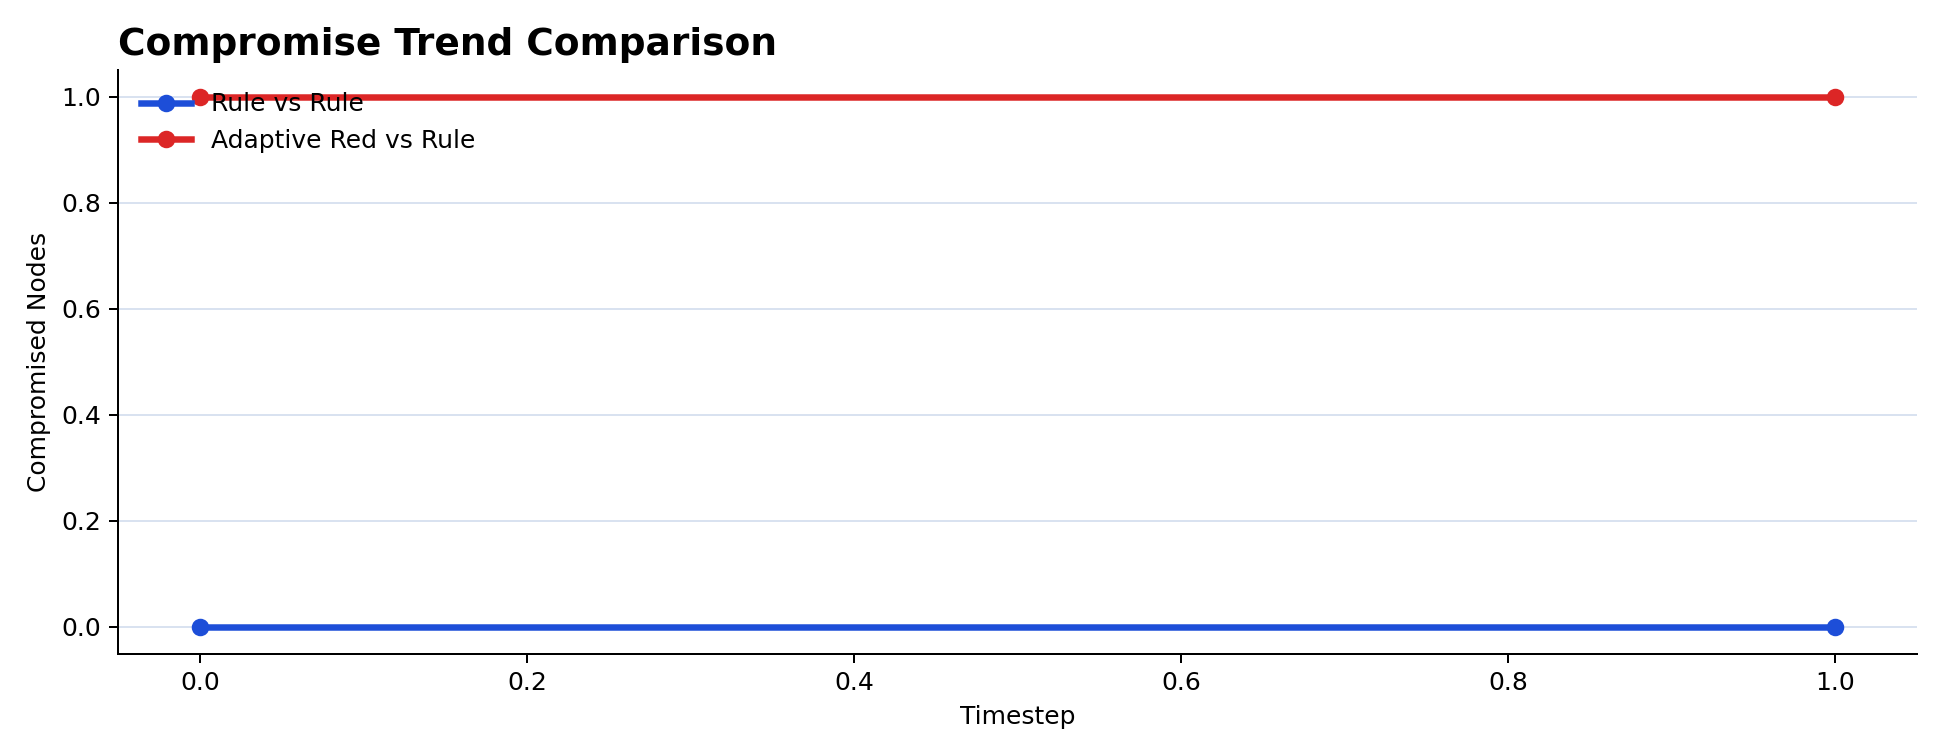
\includegraphics[width=\linewidth]{compromise_trend.png}
\caption{Compromise trend reported for the baseline and adaptive-Red comparison.}
\label{fig:trend}
\end{figure}

\begin{figure}[t]
\centering
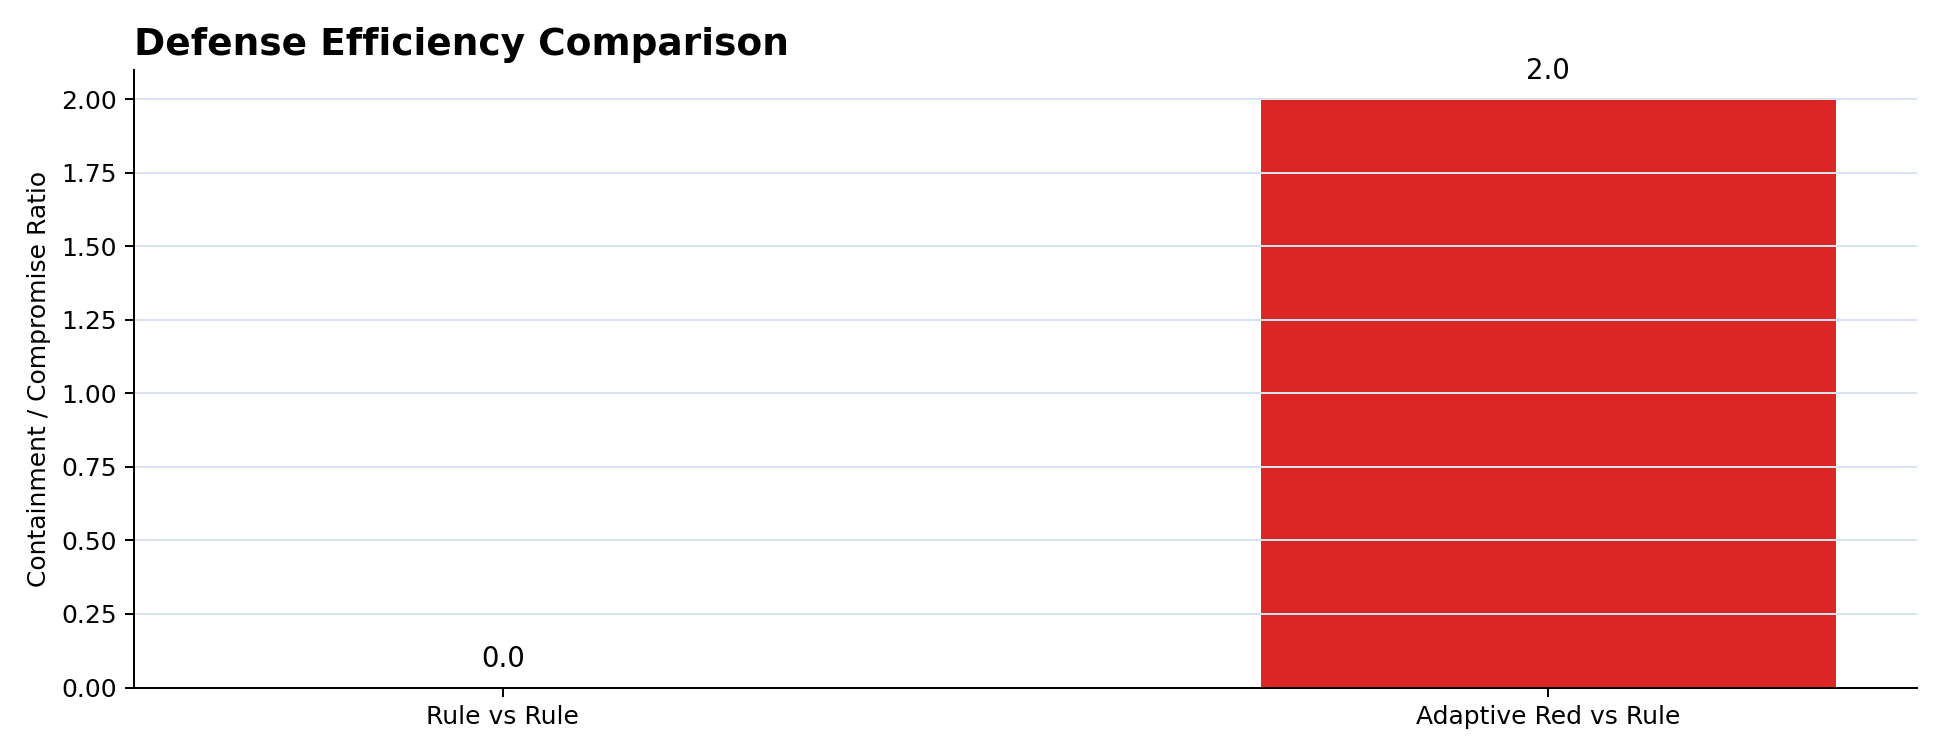
\includegraphics[width=\linewidth]{defense_efficiency.png}
\caption{Defense-efficiency view based on containment-to-compromise behavior.}
\label{fig:defense}
\end{figure}

\begin{figure}[t]
\centering
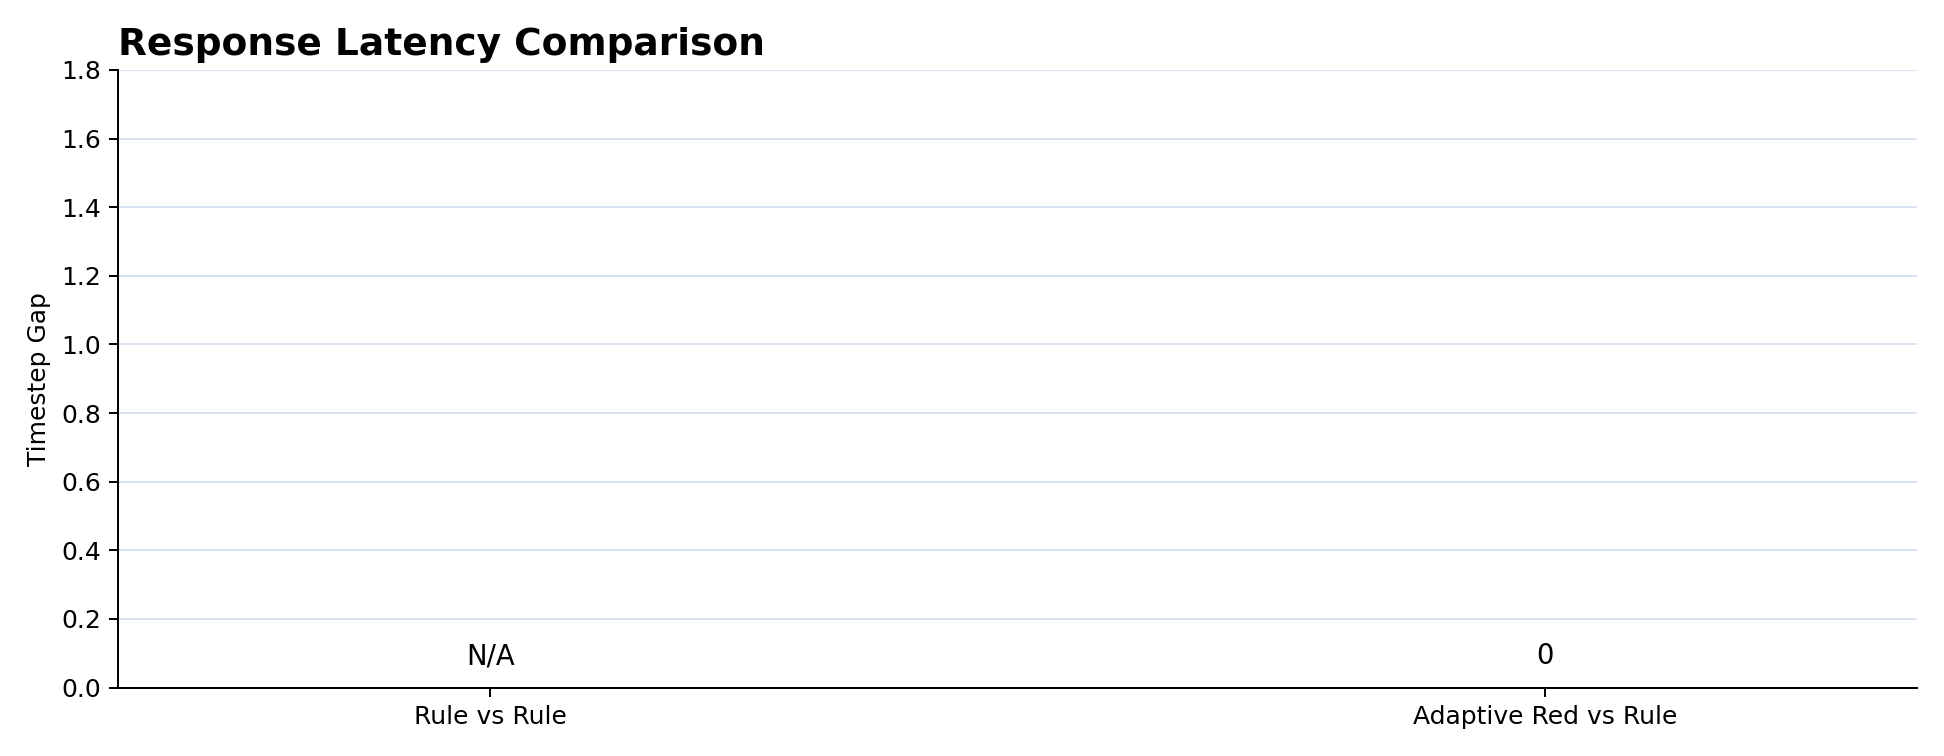
\includegraphics[width=\linewidth]{response_latency.png}
\caption{Response-latency comparison. The baseline has no containment event, while adaptive Red versus rule Blue triggers containment at timestep 0.}
\label{fig:latency}
\end{figure}

The stress-test suite compares two profiles. The Scale Scenarios Stress profile covers three scenarios over two seeds with baseline final compromised mean 0.667. The Noise and Observability Constraints profile covers two scenarios over two seeds, includes ablations, and reports baseline final compromised mean 1.0 with combined observability penalty 0.0. In the tested scope, scenario complexity produced a more visible effect than the observability proxy.

\section{Discussion}
The results are intentionally modest but useful. MARBTS is not claiming real-world exploit realism; it is demonstrating that a safe and deterministic simulator can expose policy differences, produce repeatable artifacts, and make each run auditable. The rule baseline acts as a control. Adaptive Red creates more pressure in the same scenario, and Blue containment is visible when the rule Blue policy selects block actions.

Several limitations remain. First, the baseline scenarios are small, so reported means should not be interpreted as broad security guarantees. Second, scan and monitor actions are currently informational in the kernel, meaning detection-state evolution is present in the data model but not yet a rich sensing process. Third, the adaptive planner is heuristic in the checked configuration, with external model routing disabled by default. These limits are acceptable for the submitted project stage, but they also define the clearest next steps.

\section{Conclusion and Future Work}
MARBTS delivers a safe, modular, and explainable Red/Blue simulation platform for coursework-scale cyber-defense experimentation. The project includes graph-based scenarios, legal-action enforcement, rule and adaptive policies, a turn-based kernel, observability artifacts, metrics, visualizations, multi-seed analysis, policy matrices, stress tests, ablation workflows, CLI commands, notebooks, container support, and tests.

Future work should expand the scenario library, add richer service and vulnerability semantics, make observability and deception more realistic, introduce stronger planning or reinforcement-learning policies, and provide interactive dashboards or replay tooling. A larger evaluation campaign across more varied network topologies would also make the policy comparisons more meaningful.

\begin{thebibliography}{99}

\bibitem{cip81}
S. Nema, S. Srivastava, A. Prakash, and S. Prajapati, ``Negotiating Multi Agent Red/Blue Team Simulator,'' CIP81 project report, Ramaiah Institute of Technology, Bengaluru, 2025--2026.

\bibitem{miller}
D. Miller, R. Alford, A. Applebaum, H. Foster, C. Little, and B. Strom, ``Automated adversary emulation: A case for planning and acting with unknowns,'' MITRE technical report, 2018.

\bibitem{caldera}
The MITRE Corporation, ``CALDERA: Automated adversary emulation platform,'' project documentation, Mar. 2025.

\bibitem{priya}
R. Priya and S. S. Chakkaravarthy, ``Cyber range: A comprehensive survey,'' \emph{Scientific Reports}, vol. 13, 2023.

\bibitem{wang}
Y. Wang, H. Li, and Y. Chen, ``Reinforcement learning for ransomware defense in enterprise networks,'' preprint, Aug. 2024.

\bibitem{javadpour}
A. Javadpour, M. H. Rezaei, and H. Homayoun, ``Cyber range and cyber security training: Concepts, applications and challenges,'' \emph{Computers \& Security}, 2024.

\bibitem{morozov}
N. Morozov, I. Sokolov, and P. Ivanov, ``Adaptive cyber-defense simulation for edge environments,'' \emph{Journal of Edge Computing}, 2024.

\bibitem{landolt}
J. Landolt, T. Nguyen, and M. Egele, ``Towards autonomous cyber defense with deception-aware agents,'' arXiv:2505.19837, May 2025.

\bibitem{xie}
R. Xie, K. Zhang, and L. Wang, ``LLM-assisted cyber operations in simulated enterprise networks,'' arXiv:2509.00678, Aug. 2025.

\bibitem{soule}
N. Soule, P. Das, and K. Brown, ``Evaluating autonomous red-blue agents under partial observability,'' arXiv:2506.04849, Jun. 2025.

\end{thebibliography}

\end{document}
